\documentclass{standalone}
\usepackage{tikz}
\usetikzlibrary{positioning}
\usepackage{subfigure}

\begin{document}

\minipage{6cm}
\begin{figure}
\subfigure{
\begin{tikzpicture}

  \node (A) {$\circ$};
  \node (U) [above of=A] {a};
  \node (U1) [above left of=U] {b};
  \node (U2) [above right of=U] {c};
  \node (B) [above right of=U1] {$\circ$};

  \draw [gray, dashed] (A) -- (U);
  \draw [line width=0.5mm, red] (U) -- (U1);
  \draw [line width=0.5mm, red] (U) -- (U2);
  \draw [gray, dashed] (U1) -- (B);
  \draw [gray, dashed] (U2) -- (B);

\end{tikzpicture}
}
\subfigure{
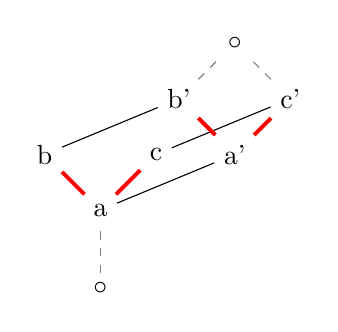
\begin{tikzpicture}

  \node (A) {$\circ$};
  \node (U) [above of=A] {a};
  \node (U1) [above left of=U] {b};
  \node (U2) [above right of=U] {c};
  \node (V) [right of=U2] {a'};
  \node (V1) [above left of=V] {b'};
  \node (V2) [above right of=V] {c'};
  \node (B) [above right of=V1] {$\circ$};

  \draw [gray, dashed] (A) -- (U);
  \draw [line width=0.5mm, red] (U) -- (U1);
  \draw [line width=0.5mm, red] (U) -- (U2);
  \draw (U) -- (V);
  \draw (U1) -- (V1);
  \draw (U2) -- (V2);
  \draw [line width=0.5mm, red] (V) -- (V1);
  \draw [line width=0.5mm, red] (V) -- (V2);
  \draw [gray, dashed] (V1) -- (B);
  \draw [gray, dashed] (V2) -- (B);
  
\end{tikzpicture}
}
\end{figure}
\endminipage

\end{document}
